\subsection{Inkjet Drucker}

\subsubsection{Vorbereitung der Polyvinylpyrrolidon-Silber-Nanopartikel}

Die Polyvinylpyrrolidon-Silber-Nanopartikel (PVP-AgNP) wurden mit einer 1ml-Spritze, durch einen Spritzenfilter (\SI{0.2}{\micro\meter}, Whataman) über eine Kanüle in die Druckerkartusche für den Inkjet-Drucker (CeraPrinter F-Series, CeraDrop) dispensiert. Die Kartusche wird mit einem Druckkopf mit 1pL-Düsen verbunden. Anschließend wurde für das Substrat die Folie aus Polyethylennaphthalat des Typs Q65HA auf die Größe A6 zugeschnitten, um die Druckplatte des Inkjet-Druckers zu bedecken. 

\subsubsection{Vorbereitung der Polyvinylpyrrolidon-Tinte}

Für die Vorbereitung der PVP-Tinte  wird ein 2:1 Gemisch von doppelt destilliertem Wasser und Triethylenglycol mit einem Gesamtvolumen von V$_{ges}$ = 3 ml hergestellt. Anschließend wird das PVP mit einer Masse von 5\% des V$_{ges}$, was einer Masse von 150 mg entspricht, mittels Feinwage eingewogen. Das PVP-Pulver in der Mischung wird durch einen Magnetrührer aufgelöst und auch hier wie bei der PVP-AgNP-Tinte in eine 1pL-Kartusche dispensiert.

\subsubsection{Inkjet Druck}

Für den Druck wird sowohl der Chuck als auch die Nozzle auf 30°C geheizt um Raumtemperaturschwankungen zu ignorieren, eine hohe Reproduzierbarkeit mit möglichst konstanten Eigenschaften zu erzielen und um Advektion beim Druck zu verhindern. Die zugeschnittene A6 Folie wird auf den Chuck gelegt und per Vakuum festgehalten. Nach Inspektion der 16 Nozzles mit Hilfe einer Kamera, ob 16 Droplets nebeneinander zu sehen sind, wird das Druck-Pattern und die Infill-Dichte der zu gedruckten Struktur analysiert, sodass der Druck aufgegeben werden kann. Nach dem Druck wird die Folie mit den gedruckten Strukturen in einem Ofen (Memmert) bei \SI{65}{\celsius} für mehrere Stunden getrocknet.

\subsubsection{Galvanisieren}

Da die Strukturen aus Silber-Nanopartikeln (AgNP) cytotoxisch sind, werden die Elektroden mit Gold beschichtet, um die Biokompabilität zu garantieren. Dafür werden auf die gedruckten Chips 300 µl einer Gold-Cyanid-Lösung (KAuCN$_2$) aufgetragen, die das komplexgebundene Gold für die Oberflächenbeschichtung enthält. In die Lösung wird  eine Referenzelektrode und eine Platinelektrode gelegt, die Gegenelektrode sind alle Silberstrukturen selbst, die über einen Sockel (IC51-390, Yamaichi) kurzgeschlossen und mit einer Krokodil-Klemme mit dem Potentiostat (VSP-300, BioLogic) verbunden sind. Für die Galvanisierung werden 12.000 Zyklen einer Pulsfolge durchgeführt. Der Puls besteht zunächst aus einer 20 ms langen Spannung von -0.9 V, gefolgt von 10 ms +0.4 V und abschließend 70 ms lang eine Spannung von 0 V. Somit dauert ein Zyklus 0.1 s, sodass ein kompletter Galvanisierungsprozess 20 Minuten benötigt. Die Pulsfolge ist in folgender Grafik abgebildet.
\begin{figure}
    \centering
    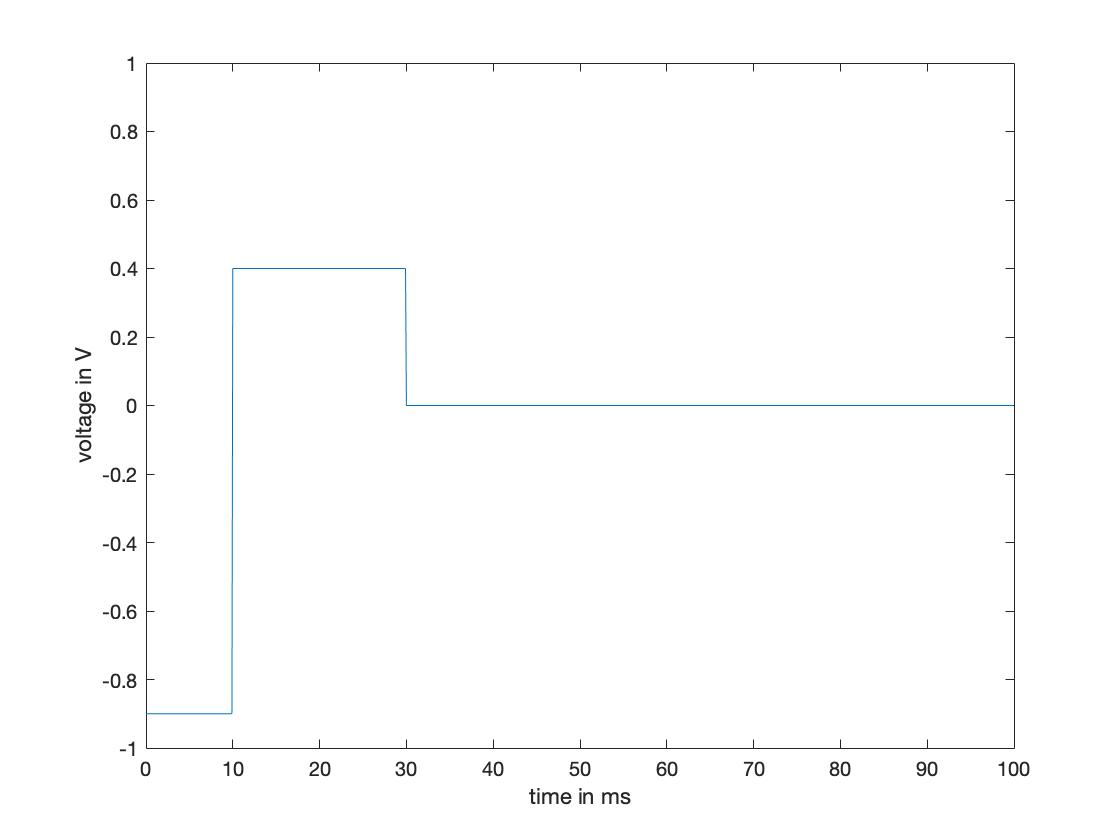
\includegraphics[width=1.0\textwidth]{img/galvanisierungpulsecurve.jpg}
    \caption{Charakteristischer Puls des Potentiostaten in einem Galvanisierungszyklus.}
    \label{fig:galvanisierung}
\end{figure}



\subsubsection{Aerosol Druck}
Um leitfähige, dreidimensionale Strukturen mittels Aerosol-Jetting zu drucken, wurde zuerst eine, auf Poly-3,4-ethylendioxythiophen polystyrolsulfonat (PEDOT:PSS) basierende, Lösung mit u.a. Carbon-Nano-Tubes (für eine verbesserte Leitfähigkeit) und Zellulose (für verbesserte mechanische Stabilität) versetzt. Nachdem Tinte und assemblierte Mechanik in den 3D-Drucker geladen waren, wurden die Drücke von Scherung, Absaugung und Atomisierung auf je \SI{600}{\ccm \per \minute}, \SI{615}{\ccm \per \minute} und \SI{15}{\ccm \per \minute} für einen kontinuierlichen, homogenen Tröpfchenstrom aus allen Nozzles geregelt.
\clearpage

